\chapter*{\uppercase{Introduction}}

Bipedal robotic walking has been well-studied for over three decades---a variety of models ranging in complexity have been studied with numerous control strategies applied in an attempt to achieve stable walking \cite{aut_2014_gcsa_01,Hurmuzlu20041647,WGCCM07}.
%
Gait generation is a common theme: some of the approaches involve passivity-based control \cite{CRTW05,SB05}, control of zero-moment point \cite{FAA10,KKKFHYH06,VB04}, hybrid zero dynamics \cite{CDG08,WGCCM07,WGK03}, central pattern generators \cite{RH02,TAT03}, and compliance-based control \cite{PDP97}.
%
The hybrid nature of bipedal walking suggest the use of the hybrid systems modeling paradigm to understand the dynamics of walking.
%
A hybrid system is a type of dynamical system which combines both continuous dynamics, treated wtih the standard equations of motion of a mechanical system operating on a normal time scale, and discrete dynamics like foot-strike which begin with a similar treatment but operate on much faster time scales.
%
The stability of solutions to traditional continuous-time systems can be understood through the use of continuous-time Lyapunov functions whereas hybrid systems are generally examined using discrete-time Lyapunov analysis in order to take into account discontinuities arising from plastic impacts.

This thesis will present a framework for improving robustness properties of hybrid systems with a special focus on bipedal robots.
%
By shaping the energy of a system to that of an associated stable limit cycle, energy shaping provides a means for improving the robustness properties of systems.
%
Due to the complex nonlinear nature of bipedal walking, the benefit of energy shaping varies from model to model.
%
It will be proven that the resulting system will be stable and that the gait will be unchanged.

The implementation utilizes the notion of control Lyapunov functions which are satisfied by construction of the proposed controller.
%
In addition, the controllers will be formulated as optimization problems using quadratic programming.
%
As a practical extension, by the nature of the formulation, the conditions of convergence can sometimes be relaxed to impose additional constraints such as torque bounding and Zero Moment Point conditions \cite{VB04}.

\section*{Overview of Energy Shaping}
Periodic behaviors in hybrid mechanical systems have specific energy signatures that evolves over time.
%
The energy dynamics of a conservative system can be understood as an interplay between kinetic and potential energy, with energy transfer occuring between these two quantities.
%
Indeed for conservative systems, the energy is constant, i.e.,
\begin{align}
  \label{eq:consys-nrg}
  E_{0} \equiv E(\q, \dq) = T(\q, \dq) + U(\q).
\end{align}
%
In a non-conservative system, this relationship does not hold, but the dynamics of energy can still be understood as
\begin{align}
  \label{eq:ncsys-nrg-cons}
  E_{0} \equiv E_{c}(\q(t), \dq(t)) = T(\q(t), \dq(t)) + U(\q(t)) - \int_{0}^{t} \! \Fnc \cdot \frac{dq(\tau)}{d\tau} \ d\tau.
\end{align}
where $\Fnc$ represents conservative forcing. Typically this represents an autonomous feedback control law and so $\Fnc : T\Q \to \R^m$ where $m$ is the number of actuators in the system.
%
As for many other control systems, the forcing from control under an autonomous feedback control is then written
\begin{align}
  \Fnc = B(q) \, u(\q, \dq).
\end{align}

From the relationship stated in \eqref{eq:ncsys-nrg-cons}, it is clear that the total energy present in the system plus the energy removed by non-conservative forcing is constant.
%
This phenomenom is well understood and it holds for all motion in mechanical systems, not just for periodic behaviors.

Understanding the energy dynamics of a system is key to the method of energy shaping.
%
By taking advantage of the presence of energy level sets in periodic behaviors, energy shaping seeks to add robustness to certain types of controllers do not necessarily have an intrinsic notion of stabilizing to a zero dynamics.
%


\section*{Hybrid Setup}
Consider a hybrid dynamical system with total energy
\begin{align*}
  E(x) &= E(\q, \dq = \frac{1}{2} \dq^{T} M(\q) \dq + U(\q).
\end{align*}
where the first term represents the kinetic energy and the second term represents the potential energy.
%
The system has coordinates $x = (\q^T, \dq^T)^T \in T\Q = \D$ which take values in the {\em domain of admissibility}, $\D$.

The discrete aspect comes from a {\em guard constraint}, $h : \Q \to \R^{+}$, which leads to a transverse plane, $\S \subset \D$, called the {\em switching surface}.
%
The uncontrolled hybrid system can be written
\begin{align}
  \Sigma = \left\{
  \begin{array}{l l}
    {\dot x} = f(x), & x \in \D \setminus \S,\\
    x^{+} = \Delta(x^{-}), &x \in \D \cap \S,
  \end{array}\right.
  \label{eq:hsys}
\end{align}
Under the action of control effort $u$, the corresponding hybrid control system has the form
\begin{align}
  \Sigma_{c} = \left\{
  \begin{array}{l l}
    {\dot x} = f(x) + g(x) \, u, & x \in \D \setminus \S,\\
    x^{+} = \Delta(x^{-}), &x \in \D \cap \S,
  \end{array}\right.
  \label{eq:csys}
\end{align}
for control values in a set $\U \subseteq \R^{m}$.
%
For the continuous dynamics, construct a Lyapunov function, $V : \D \to \R^{+}$, of the form
\begin{align}
  \label{eq:lyap}
  V(x) = \frac{1}{2} E(x)^2.
\end{align}
Consider the energy shaping controller
\begin{align}
  \label{eq:es-qp} \tag {QP}
  \mu(x, \epsilon) = \argmin_{u(x) \in \R^{n}} \ & u(x)^T u(x)\\
  \nonumber
  \mbox{s.t. } & L_{f} V(x) + L_{g} V(x) u(x) + \epsilon V(x) \leq 0.
\end{align}
Applying this to the system \eqref{eq:hsys} results in the closed-loop dynamics
\begin{align}
  \label{eq:hsys-cl}
  \Sigma = \left\{
  \begin{array}{l l}
    {\dot x} = f(x) + g(x) \, \mu(x, \epsilon), & x \in \D \setminus \S,\\
    x^{+} = \Delta(x^{-}), &x \in \D \cap \S.
  \end{array}\right.
\end{align}

\section*{Equivalence of Invariant Orbits}
In order to achieve the stated goal, it is necessary to show that, given a system with a limit cycle representing the desired behavior, energy shaping can be applied and the resulting system will have an invariant orbit which is equivalent to the nominal system. Simply put, the control contribution from the energy shaping controller must be identically zero on the orbit. Consider the following lemma:

\begin{lemma}
  Applying the energy shaping controller \eqref{eq:es-qp} to a hybrid control system \eqref{eq:csys} results in a closed-loop system that demonstrates a periodic orbit which is identical to the unshaped system \eqref{eq:hsys}.
\end{lemma}

\begin{proof}
  For states on the periodic orbit, i.e., $\xst \in \orbit$, the energy is a known constant, $E(\xst) = E_{0}$.
  %
  Therefore, the limit cycle represents an invariant level set of the energy.
  %
  By construction of the Lyapunov function \eqref{eq:lyap} used in the the controller \eqref{eq:es-qp}, it is clear that $V(\xst) = 0$ and, moreover, that $$\min_{x \in \D} V(x) = 0.$$
  %
  The solution to the optimization problem \eqref{eq:es-qp} has cost $u(x)^T u(x) = 0$ (which implies that all elements of $u(x)$ are zero) and argument $u(x) = 0$ and this satisfies the stability condition of the control Lyapunov function; indeed ${\dot V}(\xst) = 0$ since the energy does not change without external forcing.
  %
  Thus, the periodic orbits are equivalent.
\end{proof}

\section*{Stability of the Shaped System}

The next step is to prove the main idea, namely, that stability is maintained when energy shaping is applied.

\begin{theorem}
  Given an exponentially-stable limit cycle in a hybrid dynamical system of the form \eqref{eq:hsys}, application of the energy shaping controller \eqref{eq:es-qp} to the control system \eqref{eq:csys} results in the closed-loop hybrid system \eqref{eq:hsys-cl}, which is exponentially stable.
\end{theorem}

\begin{proof}
  {\em (Sketch)} Considering the energy shaping controller \eqref{eq:es-qp} with a strict equality constraint, it can be seen that the time evolution of the Lyapunov function \eqref{eq:lyap} is given by
  \begin{align*}
    \Ve(x, t) = \Ve(x_{0}, 0) \, e^{-\epsilon t}.
  \end{align*}
  From this, the limiting behavior can be examined:
  \begin{align*}
    \limeps \Ve(x, t) &= \limeps \Ve(x_{0}, 0) \, e^{-\epsilon t}\\
    &= \Ve(x_{0}, 0)\\
    &= V_0.
  \end{align*}
  The above implies that
  \begin{align*}
    \dVe(x, t) = L_{f} \Ve(x, t) + L_{g} \Ve(x, t) = 0,
  \end{align*}
  but $L_{f} \Ve(x, t) = 0$ for passive systems so it follows that
  \begin{align*}
    \limeps L_{g} \Ve(x, t) \, \mu(x, \epsilon) = 0 \Rightarrow \limeps \mu(x, \epsilon) = 0.
  \end{align*}

  It now remains to be shown that small perturbations in the input to \eqref{eq:csys} do not destabilize the system.
  %
  By the discrete converse Lyapunov Theorem, exponential stability of the discrete-time component of the hybrid system \eqref{eq:hsys} implies the existence of a discrete Lyapunov function $V : \D \cap \S \times \R^{+} \to \R^{+}$ satisfying
  %
  \begin{align*}
    c_{1} \| x \|^{2}_{\D} \leq \Vebar(x) \leq c_{2} \| x \|_{\D}^2\\
    \Vebar(\Pe(x)) - \Vebar(x) \leq c_{3} \| x \|^{2}_{\D}
  \end{align*}

  Exponential stability of the unperturbed system \eqref{eq:hsys} implies that there exists a region round the fixed point $\xst$ in which the state will converge to the limit cycle.
  %
  For simplicity, let's consider a ball of radius $\delta$, $\mathcal{B}\delta$, within this region and centered about the fixed point.
  %
  Because energy is smooth, there exists a level set of energy within this ball corresponding to the energy of the limit cycle, $E(x) = \xst$, and the guard condition applies as well, so this is a codimension-two submanifold, $\left.\S\right|_{\Es} = \{ x \in \D \cap \S | E(x) = \Es \}$.
  %
  If the system is stable within this this submanifold and the convergence of the discrete dynamics is sufficiently large to overcome divergence in the continuous dynamics due to the energy shaping controller, the exponential stability is guaranteed.


  Additionally, it should be noted that, as the perturbations approach zero, the divergence from the fixed point due the continuous dynamics approaches zero.
  %
  Thus it can be shown that sufficiently small $\epsilon$ for the energy shaping controller \eqref{eq:es-qp} applied to a system \eqref{eq:hsys} which is exponentially stable will result in exponential stability of the controlled system \eqref{eq:hsys-cl}.
\end{proof}

\begin{figure}
  \centering
  \def\svgwidth{0.5\columnwidth}
  \input{../figs/cg2d-2link-model.eps_latex}
  \caption{Compass-gait biped with Controlled Symmetries.}
  \label{fig:cg2d-model}
\end{figure}

\section*{Simulation Results}

Simulations will used to demonstrate the usefulness of the proposed control scheme.
%
As an example, consider the compass-gait biped as shown in \figref{fig:cg2d-model}.
%
This model consists of two links with five point masses and has a zero-width hip.
%
McGeer showed the compass-gait biped can walk down slopes stably in \cite{McGeer90}.
%
Later Spong and Bullo showed in \cite{SB02} that these downhill gaits can be reproduced on a fully-acutated compass-gait biped using a method styled controlled symmetries which acts to essentially rotate the frame of gravity through control.
%
As a result the compass-gait biped walking on flat ground can be modeled as a Lagrangian system of the form \eqref{eq:consys-nrg}.
%
The interplay between the kinetic energy and the shaped potential energy plays a key role in energy shaping: energy is exchanged between potential and kinetic as the robot moves, but the total energy is always conserved as can be seen in \figref{fig:nrg-cons}.


\begin{figure}
  \centering
  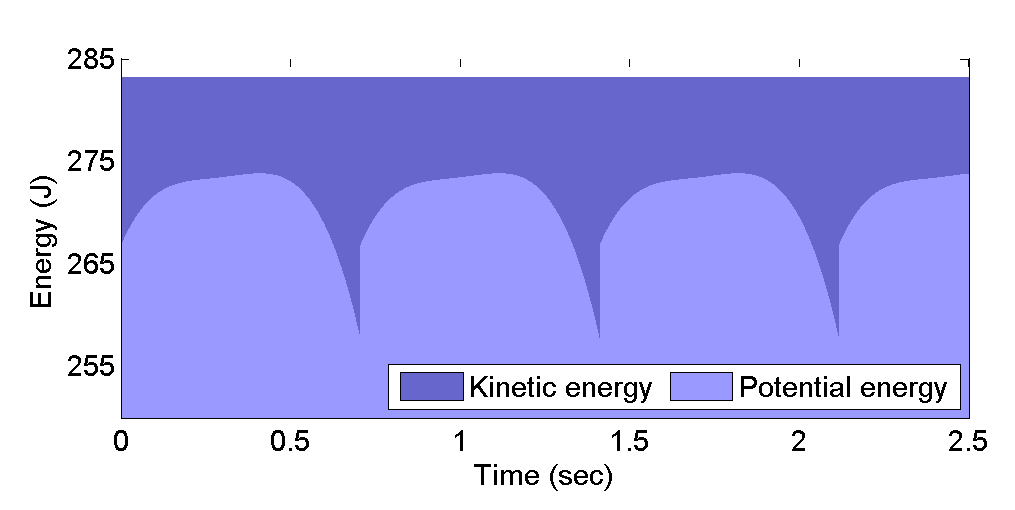
\includegraphics[width=0.85\columnwidth]{energy_cg2d_slope_model}
  \caption{Total energy of the compass-gait biped is conserved.}
  \label{fig:nrg-cons}
\end{figure}

\begin{figure}
  \centering
  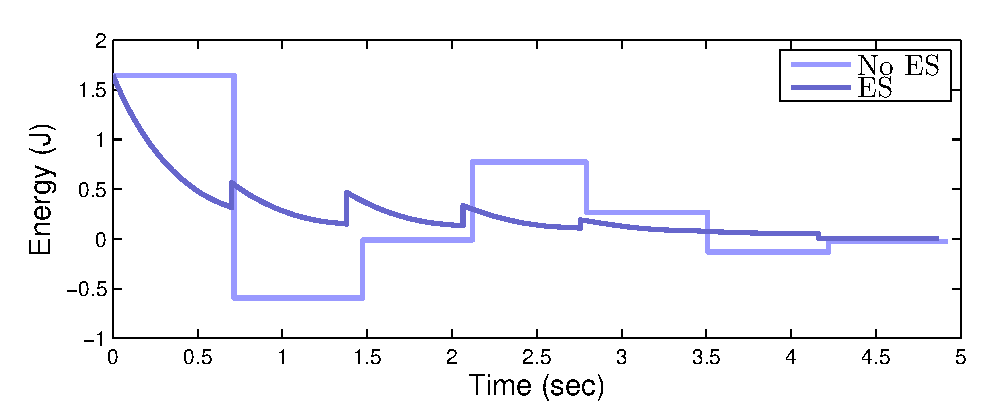
\includegraphics[width=0.85\columnwidth]{es_comparison_2link_conservative}
  \caption{Energy shaping}
  \label{fig:nrg-comp}
\end{figure}


Simulations in the research have shown that, using other forms of energy shaping, the domain of attraction is increased \cite{SpBh03}.
%
Using the proposed energy shaping controller \eqref{eq:es-qp}, the robustness of the biped can also be improved.
%
One qualitative indication of the improved robustness comes from examining the convergence of the energy to the nominal energy level.
%
\figref{fig:nrg-comp} shows that the energy convergences faster for the compass-gait biped with energy shaping applied.
%
Additionally, the convergence appears to be more uniform.
%
